\pagestyle{empty}

\cleardoublepage

\ifthenelse{\boolean{latexml}}{\chapter*{Important Formulas}}{}

\subsection*{Differentiation Rules}
\lxAddClass{diffRules}
\footnotesize
\noindent\begin{minipage}[t]{.20\linewidth}
\begin{enumerate}
\item \deriv{cx}{c}
\item	\deriv{u\pm v}{u'\pm v'}
\item	\deriv{u\cdot v}{uv'+ u'v}
\item	\deriv{\frac uv}{\frac{vu'-uv'}{v^2}}
\item	\deriv{u(v)}{u'(v)v'}
\item	\deriv{c}{0}
\item	\deriv{x}{1}
\item	\deriv{x^n}{nx^{n-1}}
\item	\deriv{e^x}{e^x}
\end{enumerate}
\end{minipage}%
\begin{minipage}[t]{.23\linewidth}
\begin{enumerate}\addtocounter{enumi}{9}
\item	\deriv{a^x}{\ln a\cdot a^x}
\item	\deriv{\ln x}{\frac{1}{x}}
\item	\deriv{\log_a x}{\frac{1}{\ln a}\cdot \frac1x}
\item	\deriv{\sin x}{\cos x}
\item	\deriv{\cos x}{-\sin x}
\item	\deriv{\csc x}{-\csc x\cot x}
\item	\deriv{\sec x}{\sec x\tan x}
\item	\deriv{\tan x}{\sec^2 x}
\item	\deriv{\cot x}{-\csc^2 x}
\end{enumerate}
\end{minipage}%
\begin{minipage}[t]{.25\linewidth}
\begin{enumerate}\addtocounter{enumi}{18}
\item	\deriv{\sin^{-1}x}{\frac{1}{\sqrt{1-x^2}}}
\item	\deriv{\cos^{-1}x}{\frac{-1}{\sqrt{1-x^2}}}
\item	\deriv{\csc^{-1}x}{\frac{-1}{|x|\sqrt{x^2-1}}}
\item	\deriv{\sec^{-1}x}{\frac{1}{|x|\sqrt{x^2-1}}}
\item	\deriv{\tan^{-1}x}{\frac{1}{1+x^2}}
\item	\deriv{\cot^{-1}x}{\frac{-1}{1+x^2}}
\item	\deriv{\cosh x}{\sinh x}
\item \deriv{\sinh x}{\cosh x}
\item \deriv{\tanh x}{\sech^2 x}
\end{enumerate}
\end{minipage}%
\begin{minipage}[t]{.25\linewidth}
\begin{enumerate}\addtocounter{enumi}{27}
\item \deriv{\sech x}{-\sech x\tanh x}
\item	\deriv{\csch x}{-\csch x\coth x}
\item	\deriv{\coth x}{-\csch^2 x}
\item	\deriv{\cosh^{-1}x}{\frac1{\sqrt{x^2-1}}}
\item	\deriv{\sinh^{-1}x}{\frac1{\sqrt{x^2+1}}}
\item	\deriv{\sech^{-1}x}{\frac{-1}{x\sqrt{1-x^2}}}
\item	\deriv{\csch^{-1}x}{\frac{-1}{|x|\sqrt{1+x^2}}}
\item	\deriv{\tanh^{-1}x}{\frac1{1-x^2}}
\item	\deriv{\coth^{-1}x}{\frac1{1-x^2}}
\end{enumerate}
\end{minipage}
\vspace{4\baselineskip}

\subsection*{Integration Rules}
\lxAddClass{intRules}
\noindent\begin{minipage}[t]{.30\linewidth}
\begin{enumerate}
\item	\myint{c\cdot f(x)}{c\int f(x)\ dx}
\item	\myint{f(x)\pm g(x)}{}\\
$\ds \int f(x)\ dx \pm \int g(x)\ dx$
\item	\myint{0}{C}
\item	\myint{1}{x+C}
\item	\myint{x^n}{\frac{1}{n+1}x^{n+1}+C, \ n\neq -1}\\
$\ n\neq -1$
\item	\myint{e^x}{e^x+C}
\item	\myint{a^x}{\frac{1}{\ln a}\cdot a^x+C}
\item	\myint{\frac{1}{x}}{\ln |x| + C}
\item	\myint{\cos x}{\sin x+C}
\item	\myint{\sin x}{-\cos x+C}
\end{enumerate}
\end{minipage}%
\begin{minipage}[t]{.31\linewidth}
\begin{enumerate}\addtocounter{enumi}{10}
\item	\myint{\tan x}{-\ln |\cos x|+C}
\item	\myint{\sec x}{\ln |\sec x+\tan x|+C}
\item	\myint{\csc x}{-\ln |\csc x+\cot x|+C}
\item	\myint{\cot x}{\ln |\sin x|+C}
\item	\myint{\sec^2 x}{\tan x+C}
\item	\myint{\csc^2x}{-\cot x+C}
\item	\myint{\sec x\tan x}{\sec x+C}
\item	\myint{\csc x\cot x}{-\csc x+C}
\item	\myint{\cos^2x}{\frac12x+\frac14\sin\big(2x\big)+C}
\item	\myint{\sin^2x}{\frac12x-\frac14\sin\big(2x\big)+C}
\item	\myint{\frac{1}{x^2+a^2}}{\frac1a\tan^{-1}\left(\frac xa\right)+C}
\end{enumerate}
\end{minipage}%
\begin{minipage}[t]{.38\linewidth}
\begin{enumerate}\addtocounter{enumi}{21}
\item	\myint{\frac{1}{\sqrt{a^2-x^2}}}{\sin^{-1}\left(\frac xa\right)+C}
\item	\myint{\frac{1}{x\sqrt{x^2-a^2}}}{\frac1a\sec^{-1}\left(\frac{|x|}{a}\right)+C}
\item	\myint{\cosh x}{\sinh x+C}
\item	\myint{\sinh x}{\cosh x+C}
\item	\myint{\tanh x}{\ln(\cosh x)+C}
\item	\myint{\coth x}{\ln |\sinh  x|+C}
\item	\myint{\frac{1}{\sqrt{x^2-a^2}}}{\ln\big|x+\sqrt{x^2-a^2}\big|+C}
\item	\myint{\frac{1}{\sqrt{x^2+a^2}}}{\ln\big|x+\sqrt{x^2+a^2}\big|+C}
\item	\myint{\frac{1}{a^2-x^2}}{\frac1{2a}\ln\left|\frac{a+x}{a-x}\right|+C}
\item	\myint{\frac{1}{x\sqrt{a^2-x^2}}}{\frac1a\ln\left(\frac{x}{a+\sqrt{a^2-x^2}}\right)+C}
\item	\myint{\frac{1}{x\sqrt{x^2+a^2}}}{\frac1a\ln\left|\frac{x}{a+\sqrt{x^2+a^2}}\right|+C}
\end{enumerate}
\end{minipage}
\normalsize

\clearpage

\noindent%
\begin{minipage}[t]{.53\linewidth}
\subsection*{The Unit Circle}

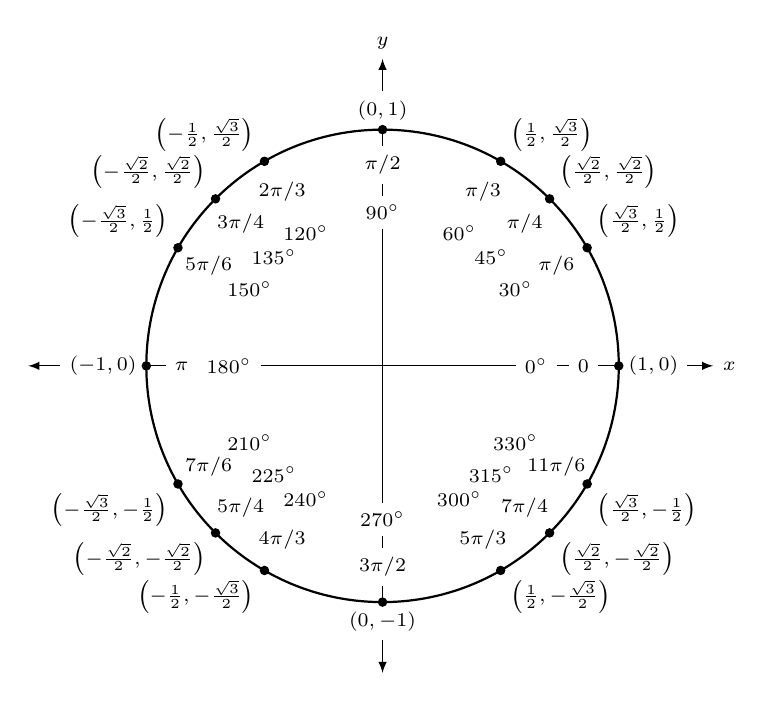
\begin{tikzpicture}[scale=3]
\draw [<->,>=latex] (-1.5,0) -- (1.4,0) node [right] {\scriptsize $x$};
\draw [<->,>=latex] (0,-1.3) -- (0,1.3) node [above] {\scriptsize $y$};
\foreach \x / \y / \z / \w / \v in {
	0/0/{1,0}/right/white,
	30/{\pi/6}/{\frac{\sqrt{3}}2,\frac 12}/above right/none,%
	45/{\pi/4}/{\frac{\sqrt{2}}2,\frac{\sqrt{2}}2}/above right/none,
	60/{\pi/3}/{\frac{1}2,\frac{\sqrt{3}}2}/{above right}/none,
	90/ {\pi/2}/{0,1}/above/white,%
	120/{2\pi/3}/{-\frac{1}2,\frac{\sqrt{3}}2}/above left/none, 
	135/{3\pi/4}/{-\frac{\sqrt{2}}2,\frac{\sqrt{2}}2}/above left/none, 
	150/ {5\pi/6}/{-\frac{\sqrt{3}}2,\frac{1}2}/above left/none,%
	180/ {\pi}/{-1,0}/left/white, 
	210/{7\pi/6}/{-\frac{\sqrt{3}}2,-\frac{1}2}/below left/none, 
	225/{5\pi/4}/{-\frac{\sqrt{2}}2,-\frac{\sqrt{2}}2}/below left/none, 
	240/{4\pi/3}/{-\frac{1}2,-\frac{\sqrt{3}}2}/below left/none,
	270/{3\pi/2}/{0,-1}/below/white, 
	300/{5\pi/3}/{\frac{1}2,-\frac{\sqrt{3}}2}/below right/none, 
	315/{7\pi/4}/{\frac{\sqrt{2}}2,-\frac{\sqrt{2}}2}/below right/none, 
	330/{11\pi/6}/{\frac{\sqrt{3}}2,-\frac{1}2}/below right/none%
}
{%
	\draw (\x:.65cm) node [fill=\v] {\scriptsize \x$^\circ$};
	\draw (\x:.85cm) node [fill=\v] {\scriptsize $\y$};
	\draw (\x:1cm) node [\w,fill=\v] {\scriptsize $\left(\z\right)$};
	\draw [fill=black] (\x:1) circle (.5pt);
}
\draw [thick] (0,0) circle (1);
\end{tikzpicture}
\end{minipage}%
%
\begin{minipage}[t]{.45\linewidth}
\subsection*{Definitions of the Trigonometric Functions}

\noindent%
\small
%\begin{minipage}[t]{.48\linewidth}
\subsubsection*{Unit Circle Definition}
%\textbf{\normalsize Unit Circle Definition}

\noindent%
\begin{minipage}{.56\linewidth}
\centering
\vskip 0in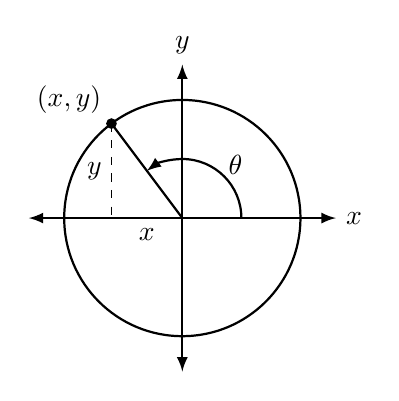
\begin{tikzpicture}[>=latex,scale=1.5,thick]
\draw [<->](-1.3,0)--(1.3,0) node [right] {$x$};
\draw [<->] (0,-1.3) -- (0,1.3) node [above] {$y$};
\draw (0,0) circle (1);
\draw [fill= black] (-.6,.8) circle (1pt);
\draw (0,0) -- (-.6,.8) node [above left] {$(x,y)$};
\draw [->] (.5,0) arc (0:127:.5);
\draw [dashed,thin] (-.6,.8) -- (-.6,0) node [pos=.5,left] {$y$};
\draw (-.3,0) node [below] {$x$};
\draw (.45,.45) node {$\theta$};
\end{tikzpicture}
\end{minipage}%
\begin{minipage}{.4\linewidth}
\small
\begin{align*}
\sin\theta &= y & \cos\theta &= x \\
\csc\theta &= \dfrac1y & \sec\theta &= \dfrac1x \\
\tan\theta &= \frac yx & \cot\theta &= \frac xy
\end{align*}
\end{minipage}
%
\subsubsection*{Right Triangle Definition}

\noindent%
\begin{minipage}{.56\linewidth}
 \centering
 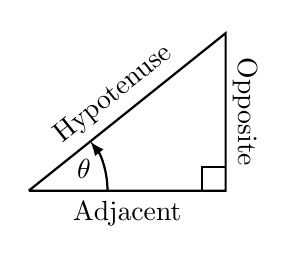
\begin{tikzpicture}[thick]
  \draw (0,0) -- (2.5,0) node [below,pos=.5] {Adjacent} -- (2.5,2) node [pos=.5,rotate=-90,shift={(0pt,7pt)}] {Opposite} -- (0,0) node [pos=.5,above,rotate=38.7] {Hypotenuse} node [shift={(20pt,8pt)}] {$\theta$};
  \draw[->,>=latex] (1,0) arc (0:38.7:1);
  \draw (2.2,0) -- (2.2,.3) -- (2.5,.3);
 \end{tikzpicture}
\end{minipage}%
\begin{minipage}{.4\linewidth}
 \small
 \begin{align*}
  \sin\theta &= \frac{\text{O}}{\text{H}} & \csc\theta &= \frac{\text{H}}{\text{O}} \\
  \cos\theta &= \frac{\text{A}}{\text{H}} & \sec\theta &= \frac{\text{H}}{\text{A}} \\
  \tan\theta &= \frac{\text{O}}{\text{A}} & \cot\theta &= \frac{\text{A}}{\text{O}}
 \end{align*}
\end{minipage}
\end{minipage}

\subsection*{Common Trigonometric Identities}

\noindent%
\begin{minipage}[t]{.25\linewidth}
	\subsubsection*{Pythagorean~Identities}
	\begin{align*}
		\sin ^2x+\cos ^2x= 1 \\
		\tan^2x+ 1 = \sec^2 x \\
		1 + \cot^2x=\csc^2 x
	\end{align*}
\end{minipage}%
\begin{minipage}[t]{.45\linewidth}
	\subsubsection*{Cofunction Identities}
	\begin{align*}
		\sin\left(\frac{\pi}{2}-x\right) &= \cos x &
		\csc\left(\frac{\pi}{2}-x\right) &= \sec x \\
		\cos\left(\frac{\pi}{2}-x\right) &= \sin x &
		\sec\left(\frac{\pi}{2}-x\right) &= \csc x \\
		\tan\left(\frac{\pi}{2}-x\right) &= \cot x &
		\cot\left(\frac{\pi}{2}-x\right) &= \tan x
	\end{align*}
\end{minipage}%
\begin{minipage}[t]{.25\linewidth}
	\subsubsection*{Double~Angle~Formulas}
	\begin{align*}
		\sin 2x &= 2\sin x\cos x \\
		\cos 2x &= \cos^2x - \sin^2 x \\
		&= 2\cos^2x-1 \\
		&= 1-2\sin^2x \\
		\tan 2x &= \frac{2\tan x}{1-\tan^2 x}
	\end{align*}
\end{minipage}

\bigskip

\noindent%
\begin{minipage}[t]{.44\linewidth}
\subsubsection*{Sum to Product Formulas}
\begin{align*}
\sin x+\sin y &= 2\sin \left(\frac{x+y}2\right)\cos\left(\frac{x-y}2\right) &~\\
\sin x-\sin y &= 2\sin \left(\frac{x-y}2\right)\cos\left(\frac{x+y}2\right) \\
\cos x+\cos y &= 2\cos \left(\frac{x+y}2\right)\cos\left(\frac{x-y}2\right) \\
\cos x-\cos y &= 2\sin \left(\frac{x+y}2\right)\sin\left(\frac{y-x}2\right)
\end{align*}
\end{minipage}%
\begin{minipage}[t]{.3\linewidth}
\subsubsection*{Power--Reducing Formulas}
\begin{align*}
\sin^2 x &= \frac{1-\cos 2x}{2} & \vphantom{\left(\frac11\right)}\\
\cos^2 x &= \frac{1+\cos 2x}{2} & \vphantom{\left(\frac11\right)}\\
\tan^2 x &= \frac{1-\cos 2x}{1+\cos 2x}
\end{align*}
\end{minipage}%
\begin{minipage}[t]{.25\linewidth}
\subsubsection*{Even/Odd Identities}
\begin{align*}
\sin(-x) &= -\sin x &~\\
\cos(-x) &= \phantom{-}\cos x \\
\tan(-x) &= -\tan x \\
\csc(-x) &= -\csc x \\
\sec(-x) &= \phantom{-}\sec x \\
\cot(-x) &= -\cot x
\end{align*}
\end{minipage}

\bigskip

\noindent
\begin{minipage}[t]{.45\linewidth}
\subsubsection*{Product to Sum Formulas}
\begin{align*}
\sin x\sin y &= \frac12\big(\cos(x-y)-\cos(x+y)\big) &~\\
\cos x\cos y &= \frac12\big(\cos(x-y)+\cos(x+y)\big) \\
\sin x\cos y &= \frac12\big(\sin(x+y)+\sin(x-y)\big)
\end{align*}
\end{minipage}%
\begin{minipage}[t]{.45\linewidth}
\subsubsection*{Angle Sum/Difference Formulas}
\begin{align*}
\sin (x\pm y) &= \sin x\cos y \pm \cos x\sin y & \vphantom{\frac11}\\
\cos (x\pm y) &= \cos x\cos y \mp \sin x\sin y & \vphantom{\frac11}\\
\tan (x\pm y) &= \frac{\tan x\pm \tan y}{1\mp \tan x\tan y}
\end{align*}
\end{minipage}

\clearpage

\subsection*{Areas and Volumes}

\begin{tabular}{llll}
	{\begin{minipage}[t]{.22\linewidth}
		\subsubsection*{Triangles}
		\begin{flalign*}
			&h=a\sin\theta &\\
			&\text{Area} = \frac12bh \\
			&\text{Law of Cosines:} \\
			&c^2=a^2+b^2-2ab\cos\theta
		\end{flalign*}
		~ % to force some space between this row and the next
	\end{minipage}}
	&
	\begin{minipage}[t]{.22\linewidth}
		~\vspace{0pt}\\
		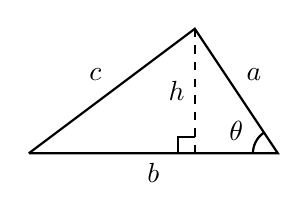
\begin{tikzpicture}[x=30pt,y=30pt,thick]
			\draw (0,0) -- node [below]  { $b$} (3,0) node [shift={(-15pt,8pt)}] {$\theta$} -- node [above right] { $a$} (2,1.5) -- node [above left] { $c$} (0,0);
			\draw (2.7,0) arc (180:125:.3);
			\draw [dashed] (2,1.5) -- (2,0) node [pos=.5,left] {$h$};
			\draw (2,.2) -- (1.8,.2) -- (1.8,0);
		\end{tikzpicture}
	\end{minipage}
	&
	{\begin{minipage}[t]{.22\linewidth}
		\subsubsection*{Right Circular Cone}
		\begin{flalign*}
			&\text{Volume} = \frac 13 \pi r^2h &\\
			&\text{Surface Area} = \\
			&\pi r\sqrt{r^2+h^2} +\pi r^2
		\end{flalign*}
	\end{minipage}}
	&
	\begin{minipage}[t]{.22\linewidth}
		~\vspace{0pt}\\
		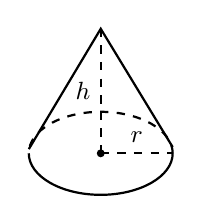
\begin{tikzpicture}[x=13pt,y=15pt,thick]
			\begin{scope}[xscale=2]
				\draw (-1,0) arc (-180:0:1);
				\draw [dashed] (1,0) arc (0:180:1);
			\end{scope}
			\draw (-2,.1) -- (0,3) -- (2,.15);
			\draw [dashed] (0,3) -- node [left] {\small $h$} (0,0);
			\draw [dashed] (0,0) -- node [above] {\small $r$} (2,0);
			\draw [fill=black] (0,0) circle (1pt);
		\end{tikzpicture}
	\end{minipage}
	\\
	\begin{minipage}[t]{.23\linewidth}
		\subsubsection*{Parallelograms}
		Area = $bh$
	\end{minipage}
	&
	\begin{minipage}[t]{.22\linewidth}
		~\vspace{0pt}\\
		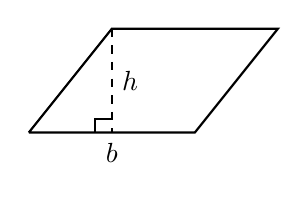
\begin{tikzpicture}[x=30pt,y=25pt,thick]
			\draw (0,0) -- node [below]  { $b$} (2,0) -- (3,1.5) -- (1,1.5) -- (0,0);
			\draw [dashed] (1,1.5) -- node [right] {$h$} (1,0);
			\draw (.8,0) -- (.8,.2) -- (1,.2);
		\end{tikzpicture}
	\end{minipage}
	&
	{\begin{minipage}[t]{.22\linewidth}
		\subsubsection*{Right Circular Cylinder}
		\begin{flalign*}
			&\text{Volume} = \pi r^2h &\\
			&\text{Surface Area} = \\
			&2\pi rh  +2\pi r^2
		\end{flalign*}
	\end{minipage}}
	&
	\begin{minipage}[t]{.22\linewidth}
		~\vspace{0pt}\\
		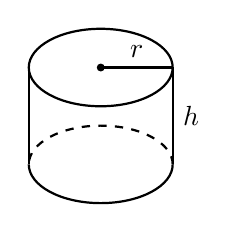
\begin{tikzpicture}[x=13pt,y=14pt,thick]
			\begin{scope}[xscale=2]
				\draw (-1,0) arc (-180:0:1);
				\draw [dashed] (1,0) arc (0:180:1);
			\end{scope}
			\draw (0,2.5) ellipse [x radius=2,y radius=1];
			\draw (-2,0) -- (-2,2.5) (2,0) -- node [right] {$h$} (2,2.5);
			\draw (0,2.5) -- node [above] {$r$} (2,2.5);
			\draw [fill=black] (0,2.5) circle (1pt);
		\end{tikzpicture}\bigskip\\~
	\end{minipage}
	\\\addlinespace[4\baselineskip]
	\begin{minipage}[t]{.23\linewidth}
		\subsubsection*{Trapezoids}
		Area = $\frac12(a+b)h$
	\end{minipage}
	&
	\begin{minipage}[t]{.22\linewidth}
		~\vspace{0pt}\\
		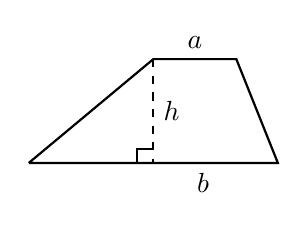
\begin{tikzpicture}[x=30pt,y=25pt,thick]
			\draw (0,0) -- node [below,pos=.7]  { $b$} (3,0) -- (2.5,1.5) -- node [above] {$a$} (1.5,1.5) -- (0,0);
			\draw [dashed] (1.5,1.5) -- node [right] {$h$} (1.5,0);
			\draw (1.3,0) -- (1.3,.2) -- (1.5,.2);
		\end{tikzpicture}\bigskip\\~
	\end{minipage}
	&
	{\begin{minipage}[t]{.22\linewidth}
		\subsubsection*{Sphere}
		\begin{flalign*}
			&\text{Volume} = \frac43\pi r^3 &\\
			&\text{Surface Area} = 4\pi r^2
		\end{flalign*}
	\end{minipage}}
	&
	\begin{minipage}[t]{.22\linewidth}
		~\vspace{0pt}\\
		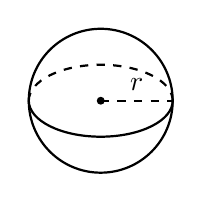
\begin{tikzpicture}[x=13pt,y=13pt,thick]
			\begin{scope}[xscale=2]
				\draw (-1,0) arc (-180:0:1);
				\draw [dashed] (1,0) arc (0:180:1);
			\end{scope}
			\draw (0,0) circle (2);
			\draw [dashed] (0,0) -- node [above] {$r$} (2,0);
			\draw [fill=black] (0,0) circle (1pt);
		\end{tikzpicture}
	\end{minipage}
	\\\addlinespace[4\baselineskip]
	{\begin{minipage}[t]{.22\linewidth}
		\subsubsection*{Circles}
		\begin{flalign*}
			&\text{Area} = \pi r^2 &\\
			&\text{Circumference} = 2\pi r
		\end{flalign*}
	\end{minipage}}
	&
	\begin{minipage}[t]{.22\linewidth}
		~\vspace{0pt}\\
		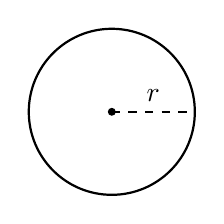
\begin{tikzpicture}[x=30pt,y=30pt,thick]
			\draw (0,0) circle (1);
			\draw [dashed] (0,0) -- node [above] {$r$} (1,0);
			\draw [fill=black] (0,0) circle (1pt);
		\end{tikzpicture}
	\end{minipage}
	&
	{\begin{minipage}[t]{.22\linewidth}
		\subsubsection*{General Cone}
		\begin{flalign*}
			&\text{Area of Base} = A &\\
			&\text{Volume} = \frac13Ah
		\end{flalign*}
	\end{minipage}}
	&
	\begin{minipage}[t]{.22\linewidth}
		~\vspace{0pt}\\
		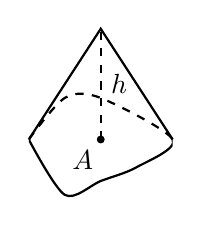
\begin{tikzpicture}[x=13pt,y=10pt,thick]
			\begin{scope}
				\clip (0,0) rectangle (4,-2.5);
				\draw [smooth] plot coordinates {(0,0) (1,1.5) (2,1.5) (4,0) (3,-1) (2,-1.5) (1,-2) (0,0)};
			\end{scope}
			\begin{scope}
				\clip (0,0) rectangle (4,2.5);
				\draw [smooth,dashed] plot coordinates {(0,0) (1,1.5) (2,1.5) (4,0) (3,-1) (2,-1.5) (1,-2) (0,0)};
			\end{scope}
			\draw (0,0) -- (2,4) -- (4,0);
			\draw [dashed] (2,0) -- node [right] {$h$}(2,4);
			\draw [fill=black] (2,0) circle (1pt);
			\draw (1.5,-.75) node {$A$};
		\end{tikzpicture}\bigskip\\~
	\end{minipage}
	\\\addlinespace[4\baselineskip]
	{\begin{minipage}[t]{.22\linewidth}
		\subsubsection*{Sectors of Circles}
		\begin{flalign*}
			&\theta \text{ in radians} &\\
			&\text{Area} = \frac12\theta r^2 \\
			&s=r\theta
		\end{flalign*}
	\end{minipage}}
	&
	\begin{minipage}[t]{.22\linewidth}
		~\vspace{0pt}\\
		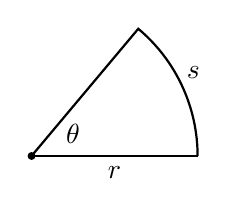
\begin{tikzpicture}[x=30pt,y=30pt,thick]
			\draw (2,0) arc (0:50:2) -- (0,0);
			\draw [] (0,0) -- node [below] {$r$} (2,0);
			\draw [fill=black] (0,0) circle (1pt);
			\draw (1.95,1.0) node {$s$};
			\draw (0,0) node [shift={(15pt,8pt)}] {$\theta$};
		\end{tikzpicture}
	\end{minipage}
	&
	{\begin{minipage}[t]{.22\linewidth}
		\subsubsection*{General Right Cylinder}
		\begin{flalign*}
			&\text{Area of Base} = A &\\
			&\text{Volume} = Ah
		\end{flalign*}
	\end{minipage}}
	&
	\begin{minipage}[t]{.22\linewidth}
		~\vspace{0pt}\\
		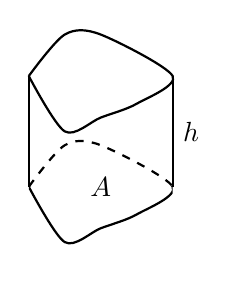
\begin{tikzpicture}[x=13pt,y=10pt,thick]
			\begin{scope}
				\clip (0,0) rectangle (4,-2.5);
				\draw [smooth] plot coordinates {(0,0) (1,1.5) (2,1.5) (4,0) (3,-1) (2,-1.5) (1,-2) (0,0)};
			\end{scope}
			\begin{scope}
				\clip (0,0) rectangle (4,2.5);
				\draw [smooth,dashed] plot coordinates {(0,0) (1,1.5) (2,1.5) (4,0) (3,-1) (2,-1.5) (1,-2) (0,0)};
			\end{scope}
			\begin{scope}[shift={(0,4)}]
				\draw [smooth] plot coordinates {(0,0) (1,1.5) (2,1.5) (4,0) (3,-1) (2,-1.5) (1,-2) (0,0)};
			\end{scope}
			\draw (0,0) -- (0,4) (4,0) -- (4,4) node [pos=.5,right] {$h$};
			\draw (2,0) node {$A$};
		\end{tikzpicture}
	\end{minipage}
\end{tabular}

\clearpage

\section*{Algebra}

\subsection*{Factors and Zeros of Polynomials}
Let $p(x) = a_n x^n + a_{n-1} x^{n-1} + \cdots + a_1 x + a_0$ be a polynomial.  If $p(a)=0$, then $a$ is a $zero$ of the polynomial and a solution
of the equation $p(x)=0$.  Furthermore, $(x-a)$ is a $factor$ of the polynomial.

\subsection*{Fundamental Theorem of Algebra}
An $n$th degree polynomial has $n$ (not necessarily distinct) zeros.  Although all of these zeros may be imaginary, a real polynomial of odd degree
must have at least one real zero.

\subsection*{Quadratic Formula}
If $p(x) = ax^2 + bx + c$, %and $0 \le b^2 - 4ac$,
then the zeros of $p$ are $x=\dfrac{-b\pm \sqrt{b^2-4ac}}{2a}$

\subsection*{Special Factoring}
\begin{flalign*}
x^2 - a^2 &= (x-a)(x+a)
&
x^3 \pm a^3 &= (x\pm a)(x^2\mp ax+a^2)
&
x^4 - a^4 &= (x^2-a^2)(x^2+a^2)
\end{flalign*}

\subsection*{Binomial Theorem}
\begin{align*}
(x+y)^2 &= x^2 + 2xy + y^2 &
(x+y)^3 &= x^3 + 3x^2y + 3xy^2 + y^3 \\
(x+y)^4 &= x^4 + 4x^3y + 6x^2y^2 + 4xy^3 + y^4 &
(x+y)^n &=\sum_{i=0}^n \binom{n}{k}x\primeskip^{n-k}y\primeskip^k
\end{align*}

\subsection*{Rational Zero Theorem}
If $p(x) = a_n x^n + a_{n-1} x^{n-1} + \dotsb + a_1 x + a_0$ has integer coefficients, then every $rational$ $zero$ of $p$ is of the form
$x=r/s$, where $r$ is a factor of $a_0$ and $s$ is a factor of $a_n$.

\subsection*{Factoring by Grouping}
$ac x^3 + adx^2 + bcx + bd = ax^2(cs+d)+b(cx+d)=(ax^2+b)(cx+d)$

\subsection*{Arithmetic Operations}
\begin{align*}
&ab+ac=a(b+c) && \frac{a}{b}+\frac{c}{d} = \frac{ad+bc}{bd} && \frac{a+b}{c} = \frac{a}{c} + \frac{b}{c} \\[.3\baselineskip]
&\frac{\left(\dfrac{a}{b}\right)}{\left(\dfrac{c}{d}\right)}=\left(\frac{a}{b}\right)\left(\frac{d}{c}\right)=\frac{ad}{bc} 
&& \frac{\left(\dfrac{a}{b}\right)}{c} = \frac{a}{bc}
&& \frac{a}{\left(\dfrac{b}{c}\right)} = \frac{ac}{b} \\[.3\baselineskip]
&a\left(\frac{b}{c}\right)= \frac{ab}{c} && \frac{a-b}{c-d}=\frac{b-a}{d-c} && \frac{ab+ac}{a}=b+c
\end{align*}

\subsection*{Exponents and Radicals}
\begin{flalign*}
&a^0=1, \; \; a \ne 0 & (ab)^x&=a^xb^x & a^xa^y &= a^{x+y} & \sqrt{a}&=a^{1/2} & \frac{a^x}{a^y}&=a^{x-y} & \sqrt[n]{a}&=a^{1/n} \\
&\left(\frac{a}{b}\right)^x=\frac{a^x}{b^x} & \sqrt[n]{a^m}&=a^{m/n} & a^{-x}&=\frac{1}{a^x} & \sqrt[n]{ab}&=\sqrt[n]{a}\sqrt[n]{b} &
(a^x)^y&=a^{xy} & \sqrt[n]{\frac{a}{b}}&=\frac{\sqrt[n]{a}}{\sqrt[n]{b}}
\end{flalign*}

\clearpage

\section*{Additional Formulas}

\subsection*{Summation Formulas}

\begin{align*}
\sum^n_{i=1}{c} &= cn
&
\sum^n_{i=1}{i} &= \frac{n(n+1)}{2}
&
\sum^n_{i=1}{i\hskip1pt^2} &= \frac{n(n+1)(2n+1)}{6}
&
\sum^n_{i=1}{i\hskip1pt^3} &= \left(\frac{n(n+1)}{2}\right)^2
\end{align*}

\subsection*{Trapezoidal Rule}

\noindent$\ds\int_a^b{f(x)}\ dx \approx \frac{\Delta x}{2}\left[f(x_1)+2f(x_2) + 2f(x_3) + \dotsb + 2f(x_{n}) + f(x_{n+1})\right]$\smallskip\\
with  $\text{Error} \leq \dfrac{(b-a)^3}{12n^2}\left[ \max \abs{\fpp(x)}\right]$

\subsection*{Simpson's Rule}

\noindent$\ds\int_a^b{f(x)}\ dx \approx \frac{\Delta x}{3}\left[f(x_1)+4f(x_2) + 2f(x_3) + 4f(x_4) + \dotsb + 2f(x_{n-1}) + 4f(x_{n}) + f(x_{n+1})\right] 
$\smallskip\\
with $\text{Error} \leq \dfrac{(b-a)^5}{180n^4}\left[ \max \abs{f\primeskip^{(4)}(x)}\right]$\bigskip\bigskip

\noindent
\begin{tabular}{ll}
 \begin{minipage}[t]{.4\linewidth}
  \subsection*{Arc Length}
  $\ds L = \int_a^b{\sqrt{1+ f\,'(x)^2}}\ dx$\bigskip\\~
 \end{minipage}
 &
 % also add volume of revolution, or nothing at all
% \begin{minipage}[t]{.4\linewidth}
%  \subsection*{Surface of Revolution}
%  $\ds S = 2\pi \int_a^b{f(x) \sqrt{1+ f\,'(x)^2}}\ dx  $\smallskip\\
%  {\small (where $f(x)\geq 0$)}\medskip\\
%  $\ds S = 2\pi \int_a^b{x \sqrt{1+ f\,'(x)^2}}\ dx 
%  $\smallskip\\
%  {\small (where $a,b \geq 0$)}\bigskip\\~
% \end{minipage}
 \\
 \begin{minipage}[t]{.4\linewidth}
  \subsection*{Work Done by a Variable Force}
  $\ds W = \int_a^b{F(x)}\ dx$
 \end{minipage}
 &
 \begin{minipage}[t]{.4\linewidth}
  \subsection*{Force Exerted by a Fluid}
  $\ds F = \int_a^b{w\,d(y)\,\ell(y)}\ dy$
 \end{minipage}
\end{tabular}

\bigskip

\subsection*{Taylor Series Expansion for $f(x)$}
\noindent$\ds p_n(x) = f(c) + \fp(c)(x-c) + \frac{\fpp(c)}{2!}(x-c)^2 + \frac{f\,'''(c)}{3!}(x-c)^3 + \dotsb + \frac{f\,^{(n)}(c)}{n!}(x-c)^n$
\bigskip

%\subsection*{Maclaurin Series Expansion for $f(x)$} %{, where $c=0$}
%\noindent$\ds p_n(x) = f(0) + \fp(0)x + \frac{\fpp(0)}{2!}x^2 + \frac{f\,'''(0)}{3!}x^3 + \dotsb + \frac{f\,^{(n)}(0)}{n!}x^n$

\clearpage

\subsection*{Summary of Tests for Series}

\begin{center}
\addtolength{\tabcolsep}{6pt}
\begin{tabular}{ccccc}

\toprule
Test & Series & \parbox{1in}{\centering Condition(s) of Convergence} & \parbox{1in}{\centering Condition(s) of Divergence} & Comment \\\midrule

$n^{\text{th}}$-Term & $\ds\sum_{n=1}^\infty a_n$ &  & $\displaystyle{\lim_{n \to \infty} a_n \neq 0}$ & \parbox{1in}{\centering cannot show convergence.}\\[3\defaultaddspace]

\parbox{.7in}{\centering Geometric\\Series} & $\ds\sum_{n=0}^\infty ar\primeskip^n$ & $ \abs{r}< 1$ & $\abs{r}\geq 1$ & Sum $=\dfrac a{1-r}$ \\[6\defaultaddspace]

\parbox[t]{.7in}{\centering Telescoping\\Series} & $\ds\sum_{n=1}^\infty b_n-b_{n+m}$ & $\ds{\lim_{n \to \infty} b_n = L}$ & & \parbox[t]{1in}{\centering Sum $=$\\$\ds\left(\sum_{n=1}^m b_n\right)-L$} \\\addlinespace

$p$-Series & $\ds\sum_{n=1}^\infty(an+b)^{-p}$ & $p>1$ & $p\leq 1$ & \\[3\defaultaddspace]

\parbox[t]{.7in}{\centering Integral\\Test} & $\ds\sum_{n=1}^\infty a_n$ & \parbox[t]{1in}{\centering$\ds\int_1^\infty a(n)\ dn$\smallskip\\ converges} & \parbox[t]{1in}{\centering$\ds\int_1^\infty a(n)\ dn$\smallskip\\ diverges} & \parbox[t]{1in}{\centering $a_n = a(n)$ must be continuous and decreasing} \\[6\defaultaddspace]

\parbox[t]{.7in}{\centering Direct\\Comparison} & $\ds\sum_{n=1}^\infty a_n$ & \parbox[t]{1in}{\centering$\ds\sum_{n=0}^\infty b_n $\smallskip\\converges and\smallskip\\$0\leq a_n\leq b_n$}
& \parbox[t]{1in}{\centering$\ds\sum_{n=0}^\infty b_n $\smallskip\\diverges and\smallskip\\$0\leq b_n\leq a_n$} & \\[12\defaultaddspace]

\parbox[t]{.7in}{\centering Limit\\Comparison} & $\ds\sum_{n=1}^\infty a_n$ & \parbox[t]{1.3in}{\centering$\ds\sum_{n=0}^\infty b_n $\smallskip\\converges and\smallskip\\$\displaystyle \lim_{n\to\infty} a_n/b_n \geq 0$}
& \parbox[t]{1in}{\centering$\ds\sum_{n=0}^\infty b_n $\smallskip\\diverges and\begin{align*}\lim_{n\to\infty} a_n/b_n &> 0\\\text{or }&=\infty\end{align*}} \\

Ratio Test & $\ds\sum_{n=1}^\infty a_n$ & \parbox{1in}{\centering$\ds\lim_{n\to\infty} \frac{a_{n+1}}{a_n}  < 1$}
& \parbox{1in}{\begin{align*}\lim_{n\to\infty} \frac{a_{n+1}}{a_n} &> 1\\\text{or } &=\infty\end{align*}} & 
\parbox{1in}{\centering $\{a_n\}$ must be positive}\\

Root Test & $\ds\sum_{n=1}^\infty a_n$ & \parbox{1in}{\centering$\ds\lim_{n\to\infty} \big(a_n\big)^{1/n} < 1$}
& \parbox{1.2in}{\begin{align*}\lim_{n\to\infty} \big(a_n\big)^{1/n} &> 1\\\text{or } &=\infty\end{align*}} & 
\parbox{1in}{\centering $\{a_n\}$ must be positive}\\\bottomrule

\end{tabular}

\end{center}
